\documentclass[
    language=english,
    doctype=technical-report,
    institution=none,
    titlestyle=book,
    oneside,
]{../../omnilatex}

\RequirePackage{config/document-settings}

\addbibresource{../../bib/bibliography.bib}

\begin{document}

\maketitle

\tableofcontents

%=============================================================================
\chapter{Introduction}
\label{sec:introduction}
%=============================================================================

This design document proposes a comprehensive redesign of the DataPipe web
dashboard. The current dashboard, launched in 2023, has grown organically
and suffers from information overload, inconsistent navigation, and poor
mobile responsiveness. This redesign addresses these issues while
introducing new capabilities for pipeline monitoring and management.

\section{Design Goals}

\begin{enumerate}
    \item Reduce the number of clicks required to reach critical
        information from 5 to 2.
    \item Support responsive layouts for desktop, tablet, and mobile.
    \item Improve accessibility to WCAG 2.2 AA compliance.
    \item Enable customisable dashboard layouts.
    \item Reduce cognitive load through progressive disclosure.
\end{enumerate}

\section{Target Users}

\begin{table}[htbp]
    \centering
    \caption{User personas for the dashboard redesign.}
    \label{tab:personas}
    \begin{tabular}{@{}lp{3.5cm}p{3.5cm}p{3.5cm}@{}}
        \toprule
        Persona & Goals & Pain Points & Technical Level \\
        \midrule
        Data Engineer & Monitor pipeline throughput,
            debug failures quickly & Too many screens, unclear
            error messages & High \\
        SRE On-Call & Detect and triage incidents fast &
            Alert fatigue, no mobile access & High \\
        Engineering Manager & View team-wide dashboards &
            Cannot aggregate across pipelines & Medium \\
        \bottomrule
    \end{tabular}
\end{table}

%=============================================================================
\chapter{Current State Analysis}
\label{sec:current-state}
%=============================================================================

\section{Usability Audit Findings}

A heuristic evaluation of the current dashboard revealed the following
issues:

\begin{description}
    \item[H1: Visibility of system status] Dashboard does not show overall
        system health at a glance. Users must navigate to individual
        pipeline pages.
    \item[H2: Match between system and real world] Technical jargon
        (consumer lag, backpressure) is used without explanation.
    \item[H3: User control and freedom] No undo for accidental pipeline
        stops. No way to customise the dashboard layout.
    \item[H4: Consistency and standards] Navigation patterns differ between
        pipeline, connector, and monitoring pages.
    \item[H5: Error prevention] Destructive actions (delete pipeline)
        lack confirmation dialogs.
\end{description}

\section{User Research Summary}

Interviews with 12 DataPipe users across three organisations revealed:

\begin{itemize}
    \item 83\% check pipeline status at least three times per day.
    \item 75\% have experienced alert fatigue from the current system.
    \item 67\% want mobile access for on-call scenarios.
    \item 50\% find the current navigation confusing.
\end{itemize}

%=============================================================================
\chapter{Proposed Design}
\label{sec:proposed-design}
%=============================================================================

\section{Information Architecture}

The new dashboard organises information into three tiers:

\begin{enumerate}
    \item \textbf{Overview tier:} System-wide health, active alerts, and
        key metrics at a glance.
    \item \textbf{Pipeline tier:} Individual pipeline status, throughput,
        and configuration.
    \item \textbf{Detail tier:} Record-level inspection, transform
        previews, and debugging tools.
\end{enumerate}

\section{Wireframe: Overview Dashboard}

The overview dashboard provides a single-screen view of system health:

\begin{figure}[htbp]
    \centering
    \begin{tikzpicture}[
        frame/.style={draw, thick, minimum width=14cm, minimum height=9cm,
                      rounded corners=4pt},
        widget/.style={draw, rounded corners=3pt, minimum width=3cm,
                       minimum height=2cm, text centered, font=\footnotesize,
                       fill=#1!10},
        header/.style={draw, minimum width=14cm, minimum height=0.8cm,
                       fill=blue!30, text centered, font=\small},
    ]
        \node[frame] (main) {};
        \node[header, anchor=north west] at (main.north west) {DataPipe Dashboard -- Overview};

        \node[widget=green] (status) [anchor=north west] at ([xshift=0.5cm, yshift=-1.2cm]main.north west)
            {System Health};
        \node[widget=blue] (pipelines) [right=0.5cm of status]
            {Active Pipelines};
        \node[widget=orange] (alerts) [right=0.5cm of pipelines]
            {Active Alerts};
        \node[widget=red] (throughput) [right=0.5cm of alerts]
            {Throughput};

        \node[widget=blue, minimum width=13cm, minimum height=2.5cm]
            (table) [below=0.5cm of status, yshift=-0.5cm, anchor=north west]
            {Pipeline Status Table};
        \node[widget=green, minimum width=6cm, minimum height=2cm]
            (chart1) [below=0.3cm of table, anchor=north west]
            {Throughput Chart};
        \node[widget=orange, minimum width=6cm, minimum height=2cm]
            (chart2) [right=1cm of chart1]
            {Latency Chart};
    \end{tikzpicture}
    \caption{Wireframe: Overview dashboard layout.}
    \label{fig:wireframe-overview}
\end{figure}

\section{Wireframe: Pipeline Detail View}

The pipeline detail view provides deep inspection capabilities:

\begin{figure}[htbp]
    \centering
    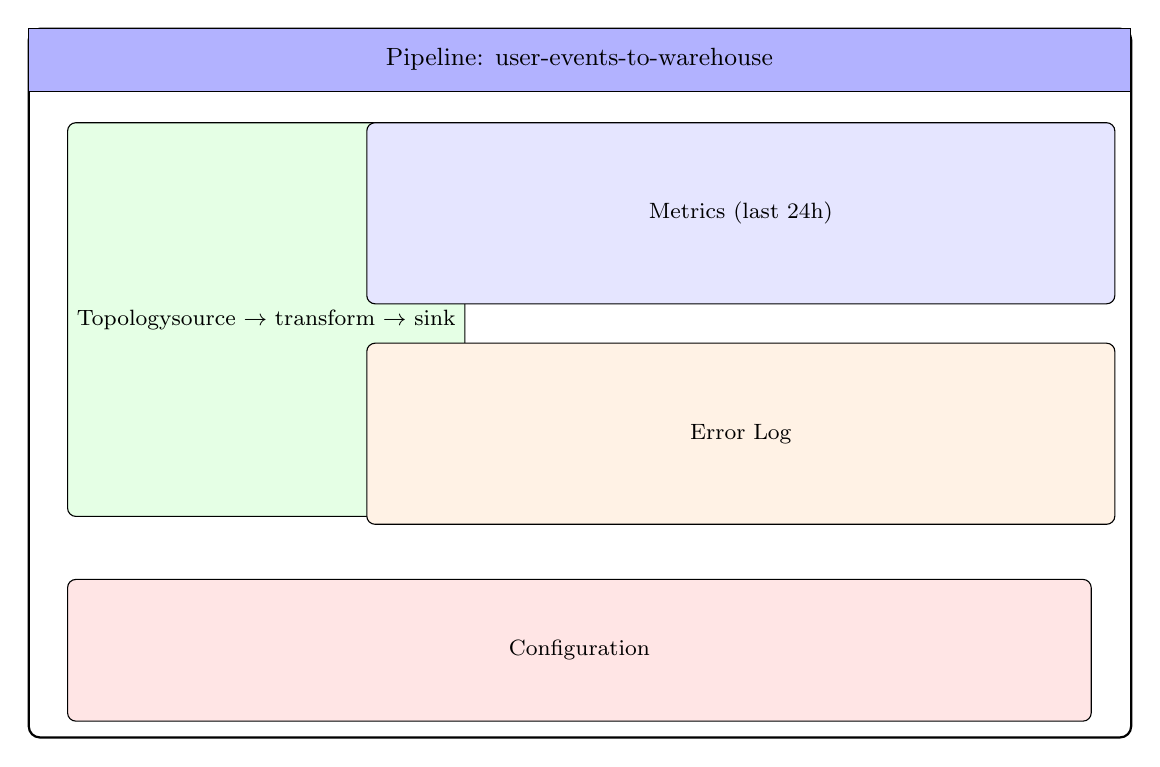
\begin{tikzpicture}[
        frame/.style={draw, thick, minimum width=14cm, minimum height=9cm,
                      rounded corners=4pt},
        widget/.style={draw, rounded corners=3pt, text centered,
                       font=\footnotesize, fill=#1!10},
    ]
        \node[frame] (main) {};
        \node[draw, minimum width=14cm, minimum height=0.8cm,
              fill=blue!30, text centered, font=\small,
              anchor=north west] at (main.north west)
            {Pipeline: user-events-to-warehouse};

        \node[widget=green, minimum width=3.5cm, minimum height=5cm,
              anchor=north west]
            at ([xshift=0.5cm, yshift=-1.2cm]main.north west)
            {Topology\\[2ex]\footnotesize source $\to$ transform $\to$ sink};
        \node[widget=blue, minimum width=9.5cm, minimum height=2.3cm,
              anchor=north west]
            at ([xshift=4.3cm, yshift=-1.2cm]main.north west)
            {Metrics (last 24h)};
        \node[widget=orange, minimum width=9.5cm, minimum height=2.3cm,
              anchor=north west]
            at ([xshift=4.3cm, yshift=-4cm]main.north west)
            {Error Log};
        \node[widget=red, minimum width=13cm, minimum height=1.8cm,
              anchor=north west]
            at ([xshift=0.5cm, yshift=-7cm]main.north west)
            {Configuration};
    \end{tikzpicture}
    \caption{Wireframe: Pipeline detail view.}
    \label{fig:wireframe-pipeline}
\end{figure}

%=============================================================================
\chapter{Interaction Design}
\label{sec:interaction}
%=============================================================================

\section{Navigation Flow}

The primary navigation follows a three-level hierarchy:

\begin{figure}[htbp]
    \centering
    \begin{tikzpicture}[
        node distance=1.2cm and 2cm,
        box/.style={draw, rounded corners, minimum width=2.5cm,
                     minimum height=0.8cm, text centered, font=\small,
                     fill=#1!20, draw=#1!60!black},
        arr/.style={->, >=stealth, thick},
    ]
        \node[box=blue]   (home)  {Overview};
        \node[box=green]  (pipe)  [below=of home] {Pipelines};
        \node[box=orange] (conn)  [left=of pipe] {Connectors};
        \node[box=purple] (mon)   [right=of pipe] {Monitoring};
        \node[box=red]    (detail)[below=of pipe] {Pipeline Detail};

        \draw[arr] (home) -- (pipe);
        \draw[arr] (home) -- (conn);
        \draw[arr] (home) -- (mon);
        \draw[arr] (pipe) -- (detail);
    \end{tikzpicture}
    \caption{Dashboard navigation hierarchy.}
    \label{fig:navigation}
\end{figure}

\section{Key Interactions}

\begin{description}
    \item[Quick actions] A floating action button provides access to
        common operations (create pipeline, view alerts, run health check)
        from any screen.
    \item[Keyboard shortcuts] Power users can navigate with keyboard:
        \texttt{g+o} for overview, \texttt{g+p} for pipelines,
        \texttt{/} to search.
    \item[Real-time updates] WebSocket connections push live metrics
        without page refresh.
    \item[Drag-to-customise] Dashboard widgets can be reordered and
        resized via drag and drop.
\end{description}

%=============================================================================
\chapter{Accessibility Requirements}
\label{sec:accessibility}
%=============================================================================

\section{WCAG 2.2 Compliance}

The redesigned dashboard must meet WCAG 2.2 Level AA. Key requirements:

\begin{table}[htbp]
    \centering
    \caption{Accessibility requirements mapped to WCAG criteria.}
    \label{tab:accessibility}
    \begin{tabular}{@{}lp{5cm}p{5cm}@{}}
        \toprule
        WCAG Criterion & Requirement & Implementation \\
        \midrule
        1.1.1 Text Alternatives & All charts have text descriptions &
            aria-label on SVG elements. \\
        1.3.1 Info and Relationships & Semantic HTML structure &
            Proper heading hierarchy, ARIA landmarks. \\
        1.4.3 Contrast & Minimum 4.5:1 contrast ratio & Design tokens
            enforce contrast. \\
        2.1.1 Keyboard & All functions accessible via keyboard &
            Focus management, keyboard event handlers. \\
        2.4.7 Focus Visible & Clear focus indicators & Custom focus
            styles via CSS. \\
        4.1.2 Name, Role, Value & ARIA attributes on interactive
            elements & Automated a11y testing in CI. \\
        \bottomrule
    \end{tabular}
\end{table}

\section{Keyboard Navigation Map}

\begin{lstlisting}[language=bash, caption={Dashboard keyboard shortcuts.}]
# Global navigation
g + o         # Go to Overview
g + p         # Go to Pipelines
g + m         # Go to Monitoring
g + c         # Go to Connectors

# Pipeline actions
Enter         # Open selected pipeline
Space         # Toggle pipeline start/stop
r             # Refresh metrics
/             # Open search
Escape        # Close modal / return to list

# Dashboard customisation
d             # Enter edit mode
Escape        # Exit edit mode
Ctrl+S        # Save layout
\end{lstlisting}

%=============================================================================
\chapter{Design System}
\label{sec:design-system}
%=============================================================================

\section{Colour Palette}

\begin{table}[htbp]
    \centering
    \caption{Colour tokens for the dashboard design system.}
    \label{tab:colours}
    \begin{tabular}{@{}llll@{}}
        \toprule
        Token & Hex & Usage & Contrast Ratio \\
        \midrule
        primary-500 & \#3B82F6 & Interactive elements & 4.6:1 on white \\
        success-500 & \#22C55E & Healthy status & 3.2:1 on white \\
        warning-500 & \#F59E0B & Warning alerts & 3.1:1 on white \\
        error-500 & \#EF4444 & Error alerts & 4.5:1 on white \\
        neutral-900 & \#111827 & Primary text & 17.4:1 on white \\
        \bottomrule
    \end{tabular}
\end{table}

\section{Typography}

\begin{itemize}
    \item \textbf{Primary:} Inter (headings and body text).
    \item \textbf{Monospace:} JetBrains Mono (code and metrics).
    \item \textbf{Scale:} 14px base, 1.25 modular scale.
\end{itemize}

\section{Component Library}

The design system includes the following reusable components:

\begin{itemize}
    \item Status badge (healthy, degraded, failed).
    \item Metric card (value, trend, sparkline).
    \item Pipeline topology diagram.
    \item Alert banner with severity indicator.
    \item Data table with sort, filter, and pagination.
    \item Modal dialog with focus trap.
    \item Toast notification (success, warning, error).
\end{itemize}

\printbibliography[heading=bibintoc, title={References}]

\end{document}
